\section{Methods}
\label{sec:Methodes}


The optimization of the films was formulated as finding the minimum mass of \iso[6]{Li} for a given detector material necessary to fulfill an interaction rate of \SI{2.5}{cps\per\nano\gram\iso[252]{Cf}} while maintaining a intrinsic gamma rejection ratio of \num{1.e-6}.

\subsection{Design Parameters}
\label{sec:DesignParameters}
The design parameters were then:
\begin{itemize}
  \item The detector material. Materials with a high \iso{6}[Li] concentration will observe more neutrons.
  \item The thickness of the detector material.
  \item The spacing of detector layers.
  \item The initial moderator thickness.
\end{itemize}

The geometry is described as follows.
There is an initial moderator of \SI{2.5}{\centi \meter} HDPE to achieve a thermal fraction around 10\%.
\footnote{The thermal energy was chosen to be \SI{5}{\electronvolt}. 
The \isotope[6]{Li} neutron cross section as this energy is 67 barns. 
A sample containing 10\% \iso[6]{Li} and a density of\SI{1.0}{\gram \per \cubic \centi\meter} would then macroscopic cross section of \SI{0.67}{\per \centi\meter}, attenuating \SI{0.67}{\percent} of the incident flux in \SI{0.01}{ \centi\meter}. 
The macroscopic cross section calculation is shown below. 
\begin{align*}
\Sigma &= \frac{\rho N_A}{M}  \left ( n_1 \sigma_1 + n_2 \sigma_2 + n_3 \sigma_3 + \dots  \right ) \\ 
       &= \frac{\rho N_A n_1 \sigma_1}{M} \\
       &= \frac{\SI{1.0}{\gram\per\cubic\centi\meter} \SI{6.022E23}{\per\mole} \SI{67}{\barn}{0.05}}{6} \\
       &= \SI{0.67}{\per\centi\meter} 
\end{align*}
}..
Following the moderator there are repeated sections of detector assembly and moderator. A single detector assembly consist of a layered film \SI{100}{\micron} thick with a light guide of \SI{0.5}{\centi\meter}.
After the absorb film and light guide assemblies is additional moderator.
Figure ~\ref{fig:GenericDetector} shows the a generic setup, while Figure ~\ref{fig:MCNPXRendering} shows the MCNPX renderings of the X-Z profile of two detector configurations.
The source is not shown as it is located \SI{2}{\meter} from the detector midpoint.
\begin{figure}
   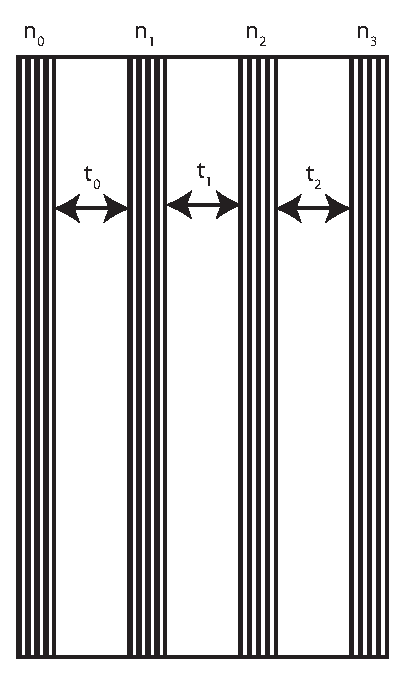
\includegraphics[width=\textwidth]{RPM8_GenericGeo}
   \caption{Generic Geometry to Optimize}
   \label{fig:GenericDetector}
\end{figure}

\begin{figure}
    \centering
    \begin{subfigure}[b]{0.45\textwidth}
        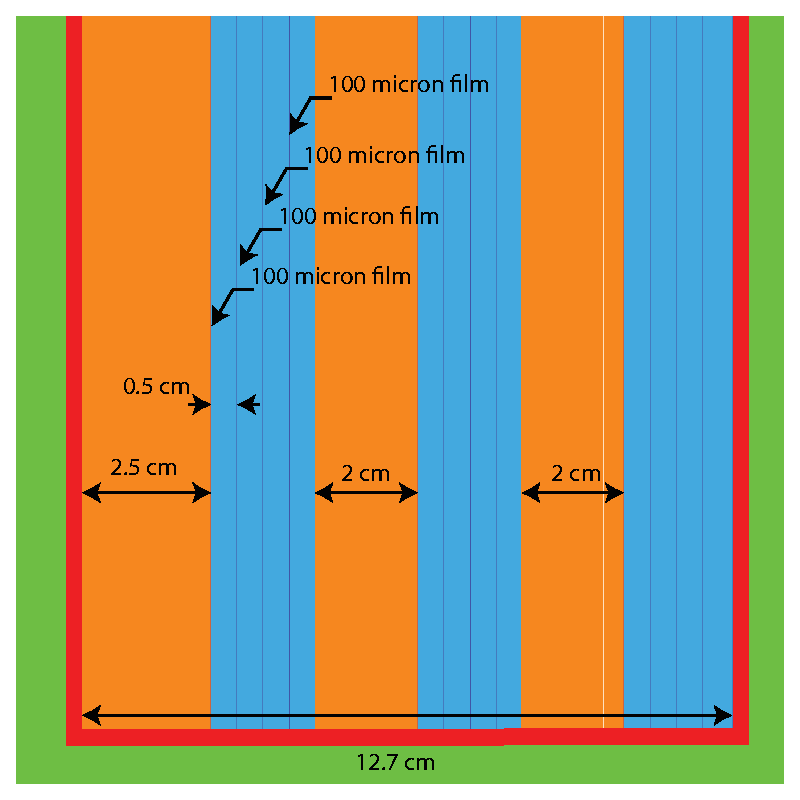
\includegraphics[width=\textwidth]{RPM8_MCNPXRender_4Assm_2cm}
        \caption{Four films per assembly with \SI{2}{\centi\meter} moderator spacing between assemblies}
    \end{subfigure}%
    ~
    \begin{subfigure}[b]{0.45\textwidth}
        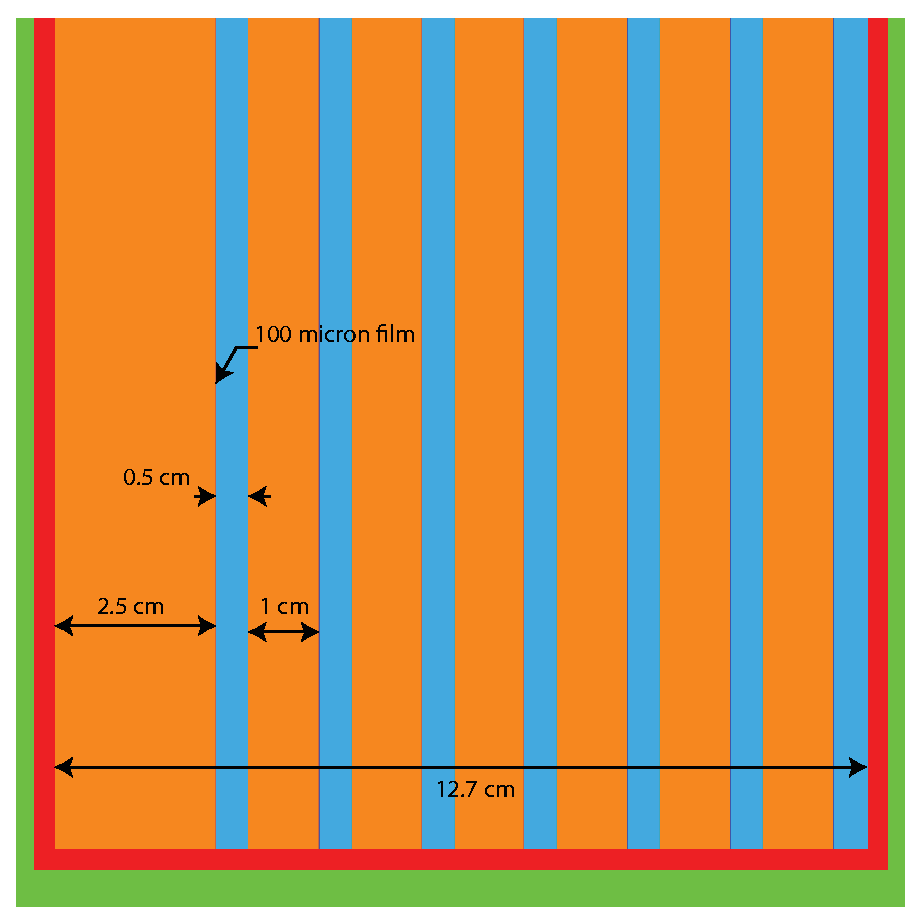
\includegraphics[width=\textwidth]{RPM8_MCNPXRender_1Assm_1cm}
        \caption{One film per assembly with \SI{1}{\centi\meter} moderator spacing between assemblies}
    \end{subfigure}
    \caption{MCNPX rendering of layered geometry}
    \label{fig:MCNPXRendering}
\end{figure}
The optimization of the detector design is presented in two parts: a numerical approach in which a matrix of detector spacing and assemblies are varied (Section ~\ref{sec:MCNPXMethods}, and a multivariate-variate optimization in which the parameters are fit to a functional form which is then optimized (Section ~\ref{sec:MVOptimization}.
\subsection{MCNPX Simulations}
\label{sec:MCNPXMethods}
A matrix of detector designs was simulated in MCNPX.
A generic script file was written (Listing ~\ref{lst:MCNPScript}) that was modified to with the code in Listing ~\ref{lst:CreateSurfaceCell} to include a user supplied number of detector assemblies, spacing between these assemblies, and initial moderator at the front of the assembly.
The MCNPX output was post processed with the python modules presented in Listing ~\ref{lst:ParseOutput} and Listing ~\ref{lst:mctal}.
See ~\ref{sec:RPM8Listings} for detailed information on the developed scripts and details on the running of the problems.

Two tallies were used in the MCNPX calculations: the interaction rate tally (tally type 4) and the surface flux tally (type 2).
If the scalar flux is defined as $\phi(\vec{r},E,t)=\int d\Omega \Phi(\vec{r},\hat{\Omega},E,t)$ the  interaction rate tally is the integral of all energies and directions of the scalar flux over a given volume, normalized by that volume ~\eqref{eqn:F4TallyDef}.
This quantity is then modified by an FM card which calculates quantities of the form $Q = C \int {\Phi(E) R_m(E) dE }$ where:
\begin{itemize}
    \item $C$ is a scalar normalization (density)
    \item $R_m(E)$ is the response function
    \item $\Phi(E)$ is the neutron flux
\end{itemize}
Similarly the surface flux is the integral over the entire surface (normalized by the surface area) of the scalar flux, as shown in \eqref{eqn:F2TallyDef}.
\begin{align}
    \label{eqn:F4TallyDef}
    \bar{\phi_V} = \frac{1}{V}\int dE \int dt \int dV \int d\Omega \AngularFlux
\end{align}
\begin{align}
    \label{eqn:F2TallyDef}
    \bar{\phi_S} = \frac{1}{A}\int dE \int dt \int dA \int d\Omega \AngularFlux
\end{align}

The FM card can modify any flux or current tally of the form $\int \psi (E) dE$ into $\int R(E)\psi(E) dE$, where $R(E)$ is the response function known to MCNP.
\subsection{1 D Transport Part}
The large detector and far away source suggest that the problem can be simplified into a one dimensional transport problem without suffering the accuracy of the solution.
As 1D deterministic transport is much faster than 3D Monte Carlo, 1D transport was explored in order to vary the problem parameters.

A matrix of \SI{25}{\percent} \iso[6]{Li} PEN films were completed with the film assemblies being 1,2,3, and 4 and with a spacing of \SI{1}{\centi\meter},\SI{2}{\centi\meter},\SI{3}{\centi\meter},and \SI{4}{\centi\meter}. 
\subsection{Multivariate Optimization}
\label{sec:MVOptimization}

The multivariate optimization problem was formulated as finding $\min_{\vec{x}} f (\vec{x})$ subject to constraints, where $f(\vec{x})$ is the response function.
